\section{Problem 1}\label{prob1}
Let us assume that the client sent the query message at \( t = 0 \). The message took \( x \) milliseconds to reach the server. Since nothing has been specified regarding the server's processing time, we assume it is negligible. The server sends the response message at \( t = x \), and the response message took \( y \) milliseconds to reach the client. The client receives the response message at \( t = x + y \). The client then takes 1 millisecond to process the message and finally sets its clock to the server's clock at \( t = x + y + 1 \). It is given that \( x \leq 2 \) and \( y \leq 2 \). (Here, all time values are with respect to a global reference time.)

% Include a figure
\begin{figure}[h]
    \centering
    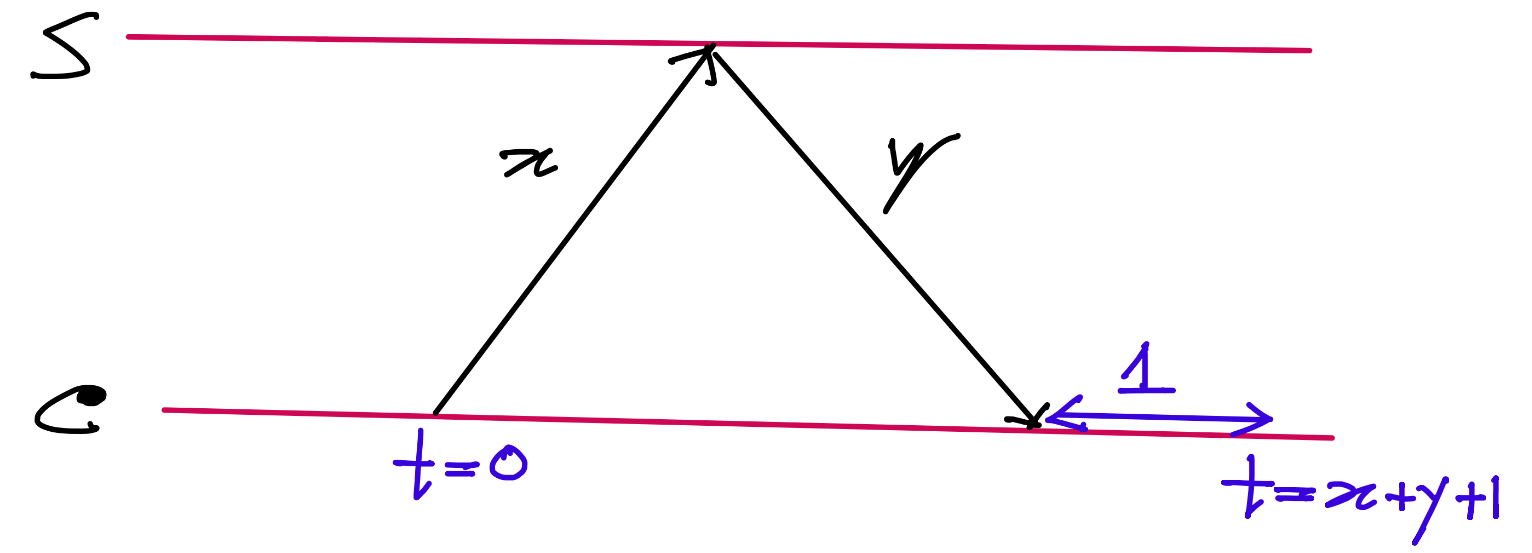
\includegraphics[width=0.5\textwidth]{IMG/Q1.jpeg}
    \caption{Timeline of Client-Server Communication}
    \label{fig:example}
\end{figure}

The server receives the query message at \( t = x \) and immediately sends the response message. The response message to the client contains only this value. Now, the client estimates the round-trip time (RTT) as:
\[
\text{RTT} = x + y + 1
\]
The client adds \( \frac{\text{RTT}}{2} \) to its clock to synchronize with the server's clock. Therefore, at \( t = x + y + 1 \), the client's clock is set to:
\[
\text{Client's Clock} = x + \frac{x + y + 1}{2}
\]
Meanwhile, the server's clock has the correct value:
\[
\text{Server's Clock} = x + y + 1
\]

The difference between the server's clock and the client's clock is given by:
\[
\text{Server's Clock} - \text{Client's Clock} = \frac{y + 1 - x}{2}
\]

This difference is maximized when \( y = 2 \) and \( x = 0 \), and minimized when \( y = 0 \) and \( x = 2 \). Therefore, the difference ranges from \( -\frac{1}{2} \) milliseconds to \( \frac{3}{2} \) milliseconds.

\begin{itemize}
    \item (a) Just after synchronization, the maximum possible difference between the server's clock and the client's clock is \( \frac{3}{2} \) milliseconds (i.e., the server's clock is ahead of the client's clock).
    \item (b) Between two synchronizations, the client's clock will run slow and drift behind the server's clock by:
    \[
    30 \times 60 \times 10^{-5} \, \text{s} = 0.018 \, \text{s} = 18 \, \text{ms}
    \]
    In the worst case, the client's clock would have already drifted behind the server's clock by \( \frac{3}{2} \) milliseconds. During the synchronization interval, it would additionally drift behind by 18 milliseconds. Thus, the maximum possible difference between the server's clock and the client's clock just before the next synchronization is:
    \[
    \frac{3}{2} + 18 = 19.5 \, \text{milliseconds}
    \]
\end{itemize}
